\chapter{問題提起}
\label{related}

本章では本研究における問題提起について述べる.

\section{ネットワーク音楽演奏における遅延}
遅延はネットワーク音楽演奏のしやすさに大きな影響を与える.
\cite{latency:effect}によると100ms以上の遅延があると演奏者は演奏が困難になる.
これらの遅延の解決を考察するためには,まずネットワーク音楽演奏における遅延を理解する必要がある.

\subsection{遅延のモデル}
この遅延を音楽演奏の文脈でどう捉えられるかを考えるためには,まずモデルを考える必要がある.
\cite{nmp:overview},\cite{latency:model}では音楽演奏は一定の拍を基準として行われているため,音楽演奏者をオシレーターと捉えている.
その場合演奏者による拍を基準とした誤差はオシレーターの周期の位相のずれとして表現できる.
これはすなわち,「演奏の崩れ」と考えることができる.
それを踏まえると,遅延がある中でのネットワーク音楽演奏においての2人の演奏者の関係は,次のような連成振動のモデルで理解することができる.

\begin{figure}
  \centering
  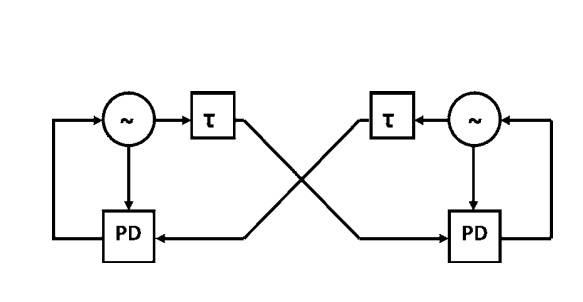
\includegraphics[width=0.8\linewidth]{src/latencymodel.png}
  \caption{連成振動のモデル.\cite{latency:model}より引用}
  \label{fig:oscillator}
\end{figure}

ここでPDはPhase Detector,すなわち演奏者の捉えた拍の感覚,\begin{math}\tau\end{math}は遅延時間である.
このモデルを踏まえて,遅延下の2人の演奏者同士が帰結するテンポは次の式であらわされる.

\begin{displaymath}
  \Omega = \frac{\omega }{1 + K\tau}
\end{displaymath}

\begin{math}\omega \end{math}は両演奏者の平均テンポ,Kは振動の状態更新を表す低数であり,\begin{math}\tau \end{math}は遅延を表す.

\subsection{遅延の原因}
遅延は\ref{background:structure}で述べたすべての工程において発生するが,特に情報の圧縮,ネットワークを介した送信において発生する.

\section{Adaptive Metronomeの問題点}
\label{related:admet}
Adaptive Metronomeは演奏者の演奏をリアルタイムで追跡し,演奏者の演奏に合わせてメトロノームのテンポを変化させるシステムを作ることに成功した.
しかし,このシステムではメトロノームに依存した演奏を行うことになり,特に遅延が大きい場合に各演奏者の演奏相手は相手の演奏者ではなく,メトロノームに必然的になってしまうと考えられる.


%%% Local Variables:
%%% mode: japanese-latex
%%% TeX-master: "./thesis"
%%% End:
